\chapter{ Analyse et planification du projet}
\renewcommand{\thesection}{\arabic{section}}
\vspace{-0.3cm}
\begin{justify}
    \section*{\texorpdfstring{Introduction}{Introduction}}
    \addcontentsline{toc}{chapter}{\textbf{Introduction}}
    \begin{justify}
    Dans ce chapitre, nous allons présenter la première phase de la méthodologie Scrum qui est la phase de planification. Il comprend l’identification des acteurs, des besoins fonctionnels et non fonctionnels, la création du diagramme de cas d’utilisation, la présentation de l’équipe de travail, l’élaboration du backlog produit, ainsi que la planification des sprints. Nous y décrivons également l’environnement logiciel et matériel adopté, ainsi que l’architecture générale retenue.
\end{justify}


    
    \section{Spécification et analyse des besoins}
        \begin{justify}
            La capture des besoins permet au client d’exprimer ses attentes. Dans cette section, nous présentons les acteurs, les besoins fonctionnels et non fonctionnels que notre solution doit respecter. 
        \end{justify}
        \subsection{Identification des acteurs}
        \begin{justify}
    Un acteur est une entité externe, qu’il s’agisse d’une personne, d’un processus ou d’un objet, qui interagit avec le système. Il exécute des tâches spécifiques et joue un rôle essentiel dans la définition des besoins du système\cite{acteur}.
    
    Dans ce projet, nous identifions 3 acteurs: 
    \begin{itemize}[label=$\bullet$]
        \item \textbf{Visiteur:} Il s’agit d’un utilisateur ordinaire qui souhaite explorer et consulter les informations disponibles sur le site. Il peut également devenir un client potentiel en s’inscrivant sur la plateforme afin d’accéder à ses fonctionnalités.
        \item \textbf{Testeur:} Son travail consiste à effectuer des test afin d’identifier l’éventuelles vulnérabilités. Il analyse ensuite les résultats obtenus, consulte les rapports générés et suit l’évolution des correctifs mis en place.
        \item \textbf{Administrateur:} est l’acteur responsable de la gestion globale du système. Ses missions incluent la gestion de l’application et des utilisateurs, la configuration des paramètres des scans ainsi que l’assurance du bon fonctionnement et de la sécurité du système.
    \end{itemize}
\end{justify} 
        \subsection{Besoins fonctionnels}
        \begin{justify}
    Les besoins fonctionnels définissent les actions attendues du système et les services à implémenter pour répondre aux attentes des utilisateurs\cite{bf}.
    
    Dans cette section, nous présentons les fonctionnalités que notre application doit assurer.
    \begin{enumerate}[left=-0.01cm]
        \item \textbf{Consulter la page d’accueil:} Accessible sans création de compte.
        \begin{itemize}[label=$\bullet$, left=-0.05cm]
            \item Parcourir la page d’accueil et consulter les sections publiques telles que la FAQ, le guide utilisateur, les services proposés, la présentation de l’équipe, la tarification, etc.
            \item Contacter l’administrateur via un formulaire de contact.
        \end{itemize}
        \item \textbf{Authentification et gestion du profil utilisateur:} Permet de gérer l’accès sécurisé à la plateforme.
            \begin{itemize}[label=$\bullet$, left=-0.05cm]
                \item S'inscrire: permettre à un utilisateur de créer un compte.
                \item Vérifier l’adresse e-mail après l’inscription: valider l'identité de l'utilisateur.
                \item S’authentifier: accéder à la plateforme via des identifiants valides.
                \item Se déconnecter: mettre fin à une session utilisateur.
                \item Réinitialiser le mot de passe en cas d’oubli: retrouver l'accès à son compte.
                \item Gérer le profil utilisateur: modifier les informations personnelles.
            \end{itemize}
        \item \textbf{Gestion des scans de tests de sécurité:} Assurer la détection automatique des vulnérabilités dans l’application web cible.
            \begin{itemize}[label=$\bullet$, left=-0.05cm]    
                \item Permettre la configuration des paramètres de scan selon les besoins spécifiques.
                \item Sélectionner les outils de sécurité à utiliser pour l’analyse.
                \item Lancer un scan de sécurité.
                \item Lancer un scan de sécurité avec authentification dynamique (cookies, jetons ou identifiants) afin de tester les parties protégées de l’application.
                \item Annuler un scan en cours : stopper un test lancé par erreur ou jugé inutile.
                \item Relancer un scan : exécuter à nouveau une analyse avec les mêmes paramètres.
                \item Planifier des scans automatiques pour une surveillance continue et garantir une sécurité régulière.
                \item Suivre la progression du scan en temps réel via WebSocket pour une visibilité immédiate de l’exécution.
                \item Visualiser les résultats du scan de sécurité: consulter les vulnérabilités détectées.
                \item Intégrer avec Jira: créer automatiquement des tickets pour les résultats critiques et assurer le suivi des incidents.
                \item Notifier via Slack: transmettre rapidement les résultats aux équipes concernées.
                \item Envoyer les résultats du scan de sécurité par e-mail: diffuser automatiquement les analyses aux parties prenantes.
                \item Gérer l’historique des rapports des scans de sécurité: conserver une trace des analyses précédentes.
                \item Téléchargement des rapports aux formats HTML, JSON, PDF, CSV et ZIP.
            \end{itemize}
        \item \textbf{Gestion des scans fonctionnels:} Vérifier  le bon fonctionnement des différentes fonctionnalités métier dans l’application web cible.
            \begin{itemize}[label=$\bullet$, left=-0.05cm]
                \item Gérer les flux de travail (scénarios de test):
                    \begin{itemize}[label=$-$, left=-0.08cm]
                        \item Créer un scénario de test: définir un parcours utilisateur à valider.
                        \item Modifier un scénario de test existant: ajuster les tests en fonction des évolutions.
                        \item Exécuter un scénario de test: déclencher le test fonctionnel.
                        \item Récupérer et afficher les scénarios de test, y compris leurs configurations et états d'exécution: assurer le suivi des tests.
                    \end{itemize}
                \item Gérer les cas de test associés à chaque scénario de test:
                    \begin{itemize}[label=$-$, left=-0.08cm]
                        \item Créer un cas de test: définir une étape précise à valider.
                        \item Modifier un cas de test existant.
                        \item Exécuter un cas de test.
                        \item Lister les cas de test: afficher tous les cas disponibles.
                        \item Récupérer et afficher les cas de test: accéder aux détails de chaque test.
                    \end{itemize}
                \item Gérer les différentes étapes associées à chaque cas de test:
                    \begin{itemize}[label=$-$, left=-0.08cm]
                        \item Créer une étape: définir une action précise à exécuter dans un cas de test.
                        \item Modifier une étape: adapter une étape existante selon les nouvelles exigences.
                        \item Supprimer une étape: retirer une action devenue obsolète ou incorrecte.
                        \item Lister les étapes d’un cas de test: afficher l’enchaînement complet des actions définies.
                        \item Récupérer et afficher les détails d’une étape: consulter les paramètres, objectifs et résultats attendus.
                    \end{itemize}
                \item Lancer un scan de test fonctionnel.
                \item Planifier des scans fonctionnels automatiques réguliers.              
                \item Relancer un scan fonctionnel : réexécuter un test fonctionnel existant.
                \item Suivre en temps réel l’exécution du scan fonctionnel via WebSocket pour une meilleure visibilité du processus.
                \item Visualiser les résultats: consulter les dysfonctionnements ou anomalies détectés.
                \item Intégrer avec Jira: création automatique de tickets pour les anomalies critiques et suivi des incidents.
                \item Notifier via Slack: transmission rapide des résultats aux équipes concernées.
                \item Envoyer les résultats du scan par e-mail: diffusion automatique des analyses fonctionnelles aux parties prenantes.
                \item Gérer l’historique des rapports des scans fonctionnels: conserver une trace des scénarios et cas de test exécutés.
                \item Téléchargement des rapports des scans fonctionnels aux différents formats.
            \end{itemize}
        \item \textbf{Gestion des scans SEO:} Évaluer la qualité de référencement et les technologies utilisées dans l’application web cible.
            \begin{itemize}[label=$\bullet$, left=-0.05cm]
                \item Lancer une analyse SEO complète (balises HTML, performance, accessibilité...).
                \item Relancer une analyse SEO : effectuer à nouveau un audit avec les mêmes critères.
                \item Identifier les technologies et frameworks utilisés.
                \item Extraire les mots-clés pertinents et analyser le contenu textuel.
                \item Générer une capture d’écran de la page cible.
                \item Calculer un score SEO global avec rapport détaillé.
                \item Suivre en temps réel l’exécution du scan SEO via WebSocket pour une meilleure visibilité du processus.
                \item Visualiser les résultats: consulter les points forts et axes d’amélioration du référencement.
                \item Intégrer avec Jira: création automatique de tickets pour les problèmes SEO majeurs et suivi des actions correctives.
                \item Notifier via Slack: transmission rapide des résultats aux équipes concernées.
                \item Envoyer automatiquement les rapports SEO par e-mail aux parties prenantes.
                \item Gérer l’historique des rapports des analyses SEO: conserver une trace des audits réalisés.
                \item Téléchargement des rapports des analyses SEO aux différents formats.
            \end{itemize}
        \item \textbf{Gestion complète des analyses (fonctionnelles, de sécurité et SEO)}: Permet l’exécution simultanée des trois types d’analyses afin d’optimiser le temps de test, de centraliser les résultats dans un seul rapport consolidé et de faciliter la corrélation entre vulnérabilités, dysfonctionnements fonctionnels et recommandations SEO.
    
        \item \textbf{Consultation des statistiques des scans via les tableaux de bord interactifs:} Offrir une visualisation graphique personnalisée des résultats pour chaque type d’utilisateur.
        \begin{itemize}[label=$\bullet$, left=-0.05cm]
            \item \textbf{Tableau de bord administrateur:} Présenter sous forme de graphiques dynamiques l’ensemble des activités de scans (fonctionnels, sécurité, SEO) classées par période, type d’analyse ou niveau de gravité, ainsi que l’état global du système.
            \item \textbf{Tableau de bord testeur:} Afficher sous forme des graphes les résultats des scans personnels, la répartition des vulnérabilités détectées, la progression des tests et la couverture fonctionnelle.
        \end{itemize}
        \item \textbf{Notifications en temps réel:} Améliorer la réactivité face aux alertes critiques.
            \begin{itemize}[label=$\bullet$, left=-0.05cm]
                \item Être notifié en temps réel des résultats pendant l’exécution des scans pour suivre en direct l’analyse.
                \item Envoyer des alertes à l'utilisateur pour les vulnérabilités critiques pour agir rapidement en cas de danger.
            \end{itemize}
        \item \textbf{Configuration des paramètres d’envoi des rapports(Email, Jira et Slack):} Permet de définir les canaux de diffusion automatisée des résultats d’analyse.
            \begin{itemize}[label=$\bullet$, left=-0.05cm]
                \item Définir les identifiants et jetons d’accès pour Slack: assurer l’envoi automatisé des rapports.
                \item Saisir les adresses e-mail des destinataires pour la diffusion des rapports.
                \item Configurer l’URL, l’identifiant du projet et les clés API pour l’intégration avec Jira.
                \item Sélectionner les types de rapports à envoyer (sécurité, fonctionnel, SEO).
                \item Choisir les formats de rapports à transmettre (HTML, PDF, JSON, etc.).
                \item Activer ou désactiver chaque canal de notification selon les préférences.
            \end{itemize}
        \item \textbf{Gestion des utilisateurs:} Assurer une administration des comptes.
            \begin{itemize}[label=$\bullet$, left=-0.05cm]
                \item Rechercher un utilisateur selon plusieurs filtres: retrouver rapidement un profil.
                \item Exporter la liste des utilisateurs: conserver une copie administrative.
                \item Consulter la liste des utilisateurs: avoir une vue globale des membres de la plateforme.
                \item Gérer les permissions des utilisateurs.
                \item Supprimer un utilisateur.
            \end{itemize}
        \item \textbf{Gestion des rapports pour l’administrateur:} Permettre à l’administrateur de superviser tous les rapports générés par les différents types de scans.
        \begin{itemize}[label=$\bullet$, left=-0.05cm]
            \item Accéder à l’ensemble des rapports de sécurité, fonctionnels et SEO générés par tous les utilisateurs.
            \item Filtrer les rapports par type d’analyse, période ou utilisateur.
            \item Rechercher un rapport spécifique.
            \item Télécharger les rapports consolidés ou individuels dans différents différents formats.
            \item Supprimer des rapports obsolètes pour maintenir une base de données claire et à jour.
        \end{itemize}
    \end{enumerate}
\end{justify}
        \subsection{Besoins non fonctionnels}
        \begin{justify}
    Les besoins non fonctionnels définissent comment le système doit fonctionner incluant les contraintes d’implémentation, d’environnement, de performance, de dépendances, de maintenance, d’extensibilité, de sécurité, de fiabilité et d’ergonomie. Une analyse approfondie de ces besoins est essentielle pour garantir la qualité globale et l’efficacité d’un produit logiciel\cite{bnf}.

    Pour optimiser l’expérience utilisateur dans ce projet, il est important de respecter les exigences de qualité suivantes:
     \begin{itemize}[label=$\bullet$, left=0.15cm]
        \item \textbf{Sécurité:} Le système doit garantir que les données des utilisateurs ainsi que les résultats des scans soient stockés de manière sécurisée. Les rapports doivent être protégés et accessibles uniquement aux utilisateurs autorisés.
        \item \textbf{Scalabilité:} Le système doit être capable de gérer une charge importante de tests effectués simultanément, sans dégradation de la performance. Il doit permettre un traitement parallèle efficace, où chaque test s'exécute de manière indépendante, garantissant que plusieurs utilisateurs puissent fonctionner simultanément sans interférer les uns avec les autres.
        \item \textbf{Fiabilité:} Le système doit être conçu pour être tolérant aux pannes et permettre une reprise automatique des scans en cas de défaillance. De plus, il doit garantir l'envoi immédiat d'alertes en temps réel lorsqu'un problème est détecté, comme des vulnérabilités critiques durant un scan, afin de permettre une réaction rapide et appropriée.
        \item \textbf{Disponibilité:} Le système doit être disponible en permanence, garantissant un fonctionnement sans interruption, 24h/24 et 7j/7.
        \item \textbf{UX/UI intuitive:} L'interface utilisateur doit être claire et ergonomique, permettant une navigation fluide et intuitive pour tous les utilisateurs. L'objectif est d'assurer une interaction simple et rapide, sans courbe d'apprentissage complexe, avec des retours immédiats lors des actions et une navigation optimisée.
        \item \textbf{Compatibilité et adaptabilité:} L'interface doit être responsive, s’adaptant de manière optimale à toutes les tailles et résolutions d’écrans, tout en offrant une expérience cohérente sur tous les navigateurs et plateformes, quel que soit l'appareil utilisé.
    \end{itemize}
\end{justify}   
    \section{Diagramme de cas d’utilisation global}
    Le diagramme de cas d'utilisation offre une vue d'ensemble du système en représentant les interactions entre les acteurs et les cas d'utilisation correspondant aux principales fonctionnalités attendues. Il permet de définir les exigences fonctionnelles, de clarifier les objectifs du projet, de délimiter le périmètre du système et d’identifier les besoins des utilisateurs \cite{case}.

Dans ce diagramme, présenté à la figure \ref{fig:UseCaseDiagram1}, sont regroupés tous les cas d’utilisation de base afin d’offrir une perspective globale du fonctionnement de notre système.
\begin{figure}[H]
\centering
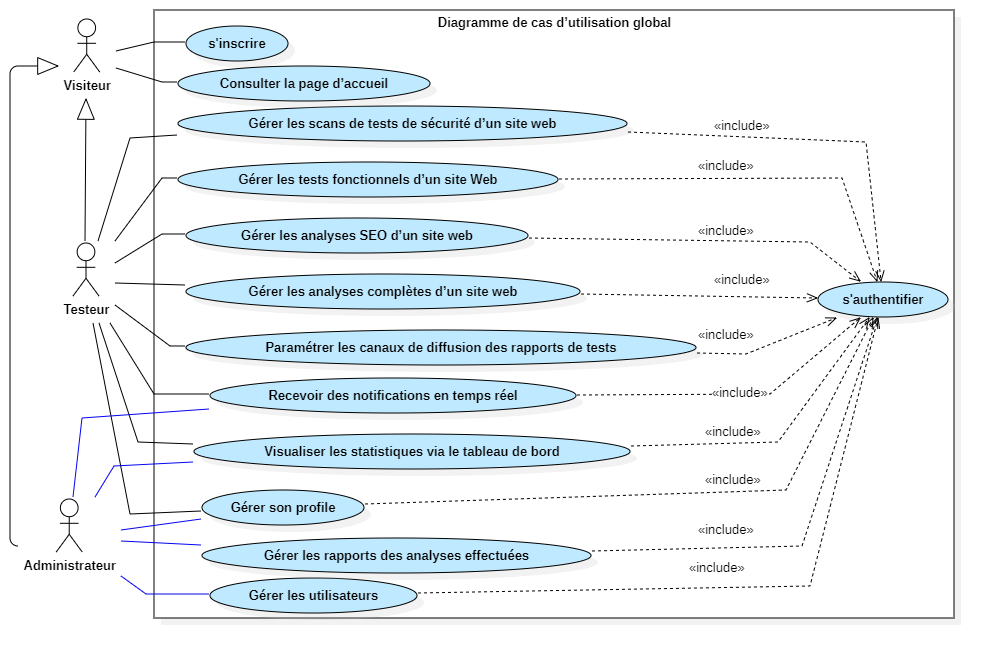
\includegraphics[width=\textwidth]{chapitres/ch2/img/global-last- use-case.png}
\caption{Diagramme de cas d'utilisation global}
\label{fig:UseCaseDiagram1}
\end{figure}
\vspace{-0.3cm}
    \section{Pilotage du projet avec Scrum}
    Cette section décrit le pilotage du projet selon la méthodologie Scrum, en présentant les outils utilisés, la composition de l’équipe et ses rôles, le backlog du produit et le découpage du projet.
\subsection{Présentation de l’équipe de travail }
La réussite du projet repose sur une bonne organisation de l’équipe et une répartition claire des rôles, assurées par la méthodologie Scrum. Dans le cadre de ce projet, les trois rôles clés de Scrum sont attribués aux membres de l’équipe de la manière suivante :
\begin{itemize}[label=$\bullet$]
    \item \textbf{Scrum Master:} Représenté par notre encadrant professionnel, Monsieur \textbf{Omar NACHMI}, qui a guidé l’équipe dans l’adoption de Scrum, assurant une organisation efficace et une amélioration continue des processus de travail.
    \item \textbf{Product Owner :}  Représenté également par Monsieur \textbf{Omar NACHMI}, qui a proposé et dirigé ce travail, en fournissant des explications approfondies sur les diverses exigences et fonctionnalités requises par le système.
    \item \textbf{Équipe de développement:} Composée de moi-même, \textbf{Rihab Cherni}, et de ma collègue \textbf{Maïssa Ben Ghalba}, nous avons travaillé ensemble pour réaliser le projet, en collaborant étroitement à chaque étape du développement.
\end{itemize}
\subsection{Outils SCRUM utilisés}
Pour le suivi de notre projet, nous avons adopté des outils collaboratifs : \textbf{OpenProject} pour la gestion des tâches et le suivi quotidien de notre progression, \textbf{Microsoft Teams} pour la communication entre les membres de l’équipe, l’organisation des réunions quotidiennes (daily meetings), des réunions RH et la coordination des sprints, et \textbf{GitLab} pour le travail collaboratif sur le code et la gestion de version.
 \subsection{Backlog du produit }
Le backlog produit représente une liste des fonctionnalités nécessaires au développement du produit. Géré par le Product Owner, il permet d'assurer l’alignement entre les besoins des utilisateurs et les objectifs du projet. Il constitue un outil de référence pour l’équipe de développement, en collaboration avec le Scrum Master et les parties prenantes \cite{backlog}.

Les epics structurent le backlog à un niveau stratégique en regroupant des fonctionnalités clés du produit. Plus génériques et moins détaillés que les user stories, ils doivent être découpés progressivement pour être développés. Ils facilitent la planification, la priorisation, la communication avec les parties prenantes et la gestion de la complexité tout au long du projet\cite{epic}.

Le tableau \ref{tab:backlog} présente le backlog produit de notre projet, en précisant pour chaque épique sa priorité, le niveau de risque, ainsi que son effort estimé en jours.
\renewcommand{\arraystretch}{1.3}
\begin{spacing}{1}
    \begin{longtable}{|p{0.35cm}|p{9.3cm}|p{1.45cm}|p{1.45cm}|p{2.4cm}|}
        \caption{Backlog produit} \label{tab:backlog} \\\hline
        \textbf{\small ID} & \textbf{\small Épics} & \textbf{\small Priorité} & \textbf{\small Risques} & \textbf{\small Estimation(j)} \\ \hline
        1  & \textbf{Initialisation du projet} & Élevée & Basse & 15 \\
        \hline
        2 & \textbf{Consultation de la page d’accueil} & Basse & Basse & 5 \\
        \hline 
        3  & \textbf{Authentification et gestion du profil} & Moyenne & Basse & 4 \\
        \hline
       4  & \textbf{Gestion des scans de tests de sécurité d’un site web} & Élevée & Élevée & 20 \\
        \hline  
        5  & \textbf{Gestion des tests fonctionnels d’un site web} & Élevée & Élevée & 15 \\
        \hline 
        6  & \textbf{Gestion des analyses SEO d’un site web} & Élevée & Moyenne & 10 \\
        \hline      
        7  & \textbf{Gestion des analyses complètes} & Élevée & Élevée & 6 \\
        \hline
        8  & \textbf{Visualisation des statistiques via le tableau de bord} & Élevée & Élevée & 8 \\
        \hline
        9  & \textbf{Notifications en temps réel} & Élevée & Basse & 2 \\
        \hline
        10 & \textbf{Paramétrage des canaux de diffusion des rapports de tests} & Moyenne & Moyenne & 2 \\ 
        \hline
        11 & \textbf{Gestion des utilisateurs} & Moyenne & Basse & 2 \\
        \hline
        12 & \textbf{Gestion des rapports des analyses effectuées } & Moyenne & Basse & 3 \\
        \hline
        13 & \textbf{Déploiement de l'application} & Moyenne & Moyenne & 5 \\
        \hline
        \multicolumn{4}{|c|}{\textbf{TOTAL}} & \textbf{97(jours)} \\
        \hline 
    \end{longtable}
\end{spacing}
\vspace{-0.1cm}
\subsection{Planification des sprints}
Pour la planification, nous avons choisi de répartir le travail en deux livraisons (releases), chacune étant divisée en deux sprints, comme indiqué dans le tableau \ref{tab:Planification}.
{\renewcommand{\arraystretch}{1.3}
\begin{table}[H]
	\begin{center}
    \caption{Planification des Livraisons et des Sprints}
    \label{tab:Planification}
	\begin{tabular}{|p{8.2cm}|p{8.2cm}|}\hline
		\textbf{Livraison 1 (Total : 50 jours)} & \textbf{Livraison 2 (Total : 47 jours)} \\\hline
		\begin{minipage}[t]{\linewidth}
            \textbf{Sprint 1.1} (26 jours) :
            \begin{itemize}[label=$-$, left=0.2cm]
                \item Initialisation du projet
                \item Consultation de la page d’accueil
                \item Authentification
                \item Gestion des utilisateurs
            \end{itemize}
            \textbf{Sprint 1.2} (24 jours) :
            \begin{itemize}[label=$-$, left=0.2cm]
                \item Gestion des scans de tests de sécurité
                \item Paramétrage des canaux de diffusion des rapports de tests
                \item Notifications en temps réel
            \end{itemize}
            \vspace{0.1cm}
        \end{minipage}
        &
        \begin{minipage}[t]{\linewidth}
            \textbf{Sprint 2.1} (25 jours) :
            \begin{itemize}[label=$-$, left=0.2cm]
                \item Gestion des scans fonctionnels
                \item Gestion des scans SEO
            \end{itemize}
            \textbf{Sprint 2.2} (22 jours) :
            \begin{itemize}[label=$-$, left=0.2cm]
                \item Gestion des scans complètes (fonctionnels, sécurité et SEO)
                \item Visualisation du tableau de bord
                \item Gestion des rapports des analyses effectuées
                \item Déploiement de l’application
            \end{itemize}
        \end{minipage}
        \\\hline
	\end{tabular}
 	\end{center}
\end{table}
}
\vspace{-0.7cm}
Cette répartition a permis d’ajuster le projet au fil des sprints tout en intégrant les fonctionnalités essentielles dès les premières étapes du développement. 
    \section{Planning prévisionnel du projet}
    Pour une gestion optimale du projet, nous avons utilisé un diagramme de Gantt, permettant de répartir les tâches de manière structurée et de visualiser leur durée ainsi que leur enchaînement. 
Comme illustré dans la figure \ref{fig:gantt}, chaque tâche est associée à un intervalle de temps précis, facilitant le suivi de l'avancement et la gestion des priorités. Cet outil aide à identifier les étapes clés et à ajuster les délais si nécessaire, garantissant ainsi une coordination efficace et un déroulement fluide du notre projet.
\begin{figure}[H]
    \centering
    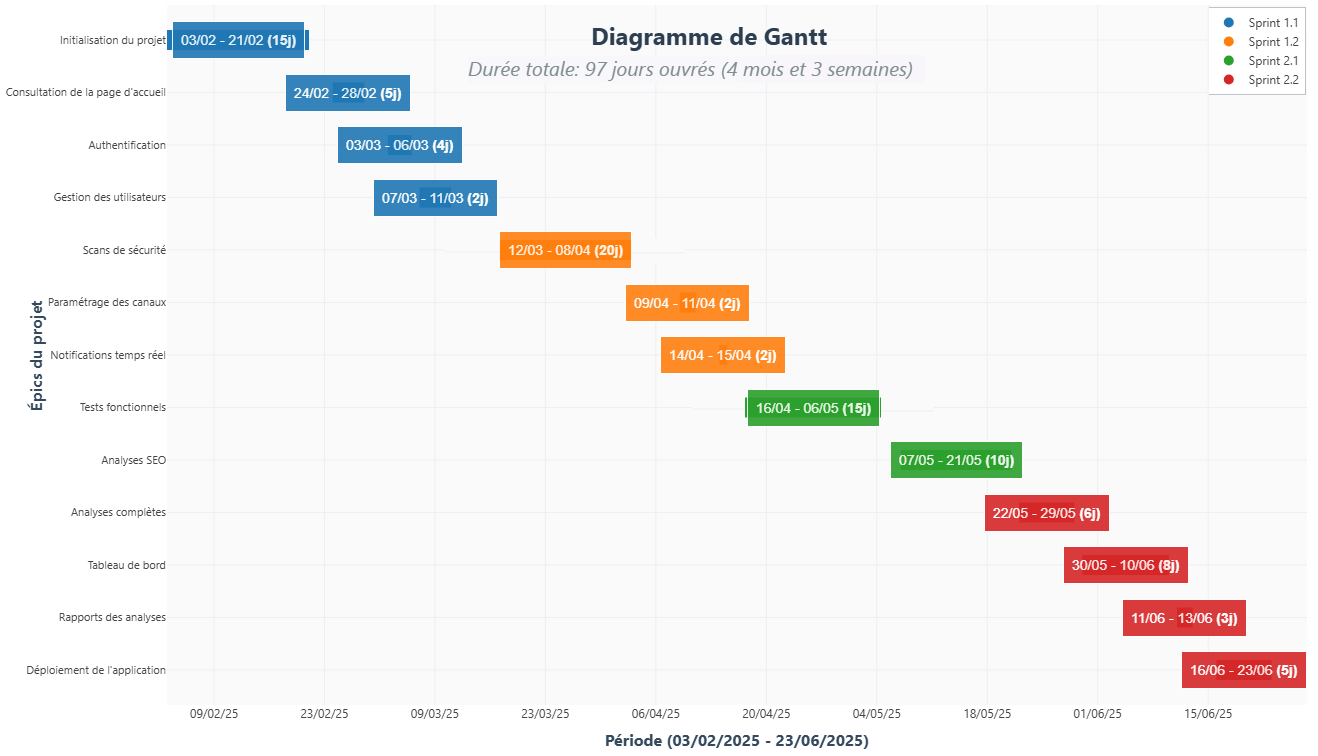
\includegraphics[width=\linewidth]{chapitres/ch2/img/gantt-last.png}
    \caption{Diagramme de Gantt}
    \label{fig:gantt}
\end{figure}
\vspace{-0.5cm}  
    \section{Rétrospective Agile}
    Dans cette section nous allons présenter les différents artefacts Scrum que nous avions utilisé pour accomplir notre projet afin de nous faciliter la gestion des tâches. 
\subsection{Scrum board}
Le Scrum board est un outil visuel utilisé pour organiser et suivre les tâches dans chaque sprint (à faire, en cours, terminées). Il permet aux équipes de suivre l'avancement du travail tout au long des sprints. Sa mise à jour est la responsabilité des membres de l’équipe, facilitant la gestion des tâches et la visualisation de la progression\cite{Scrumboard}.

Nous avons utilisé l’outil \textbf{«OpenProject»} pour organiser les tâches sous forme de cartes réparties sur quatre colonnes : à faire, en cours, à tester et terminées. Cet outil nous a permis de suivre efficacement l'avancement de nos sprints, comme illustré dans la figure \ref{fig:boardOpenProject} représentant le Scrum board du Sprint 1.
\begin{figure}[H]
    \centering
    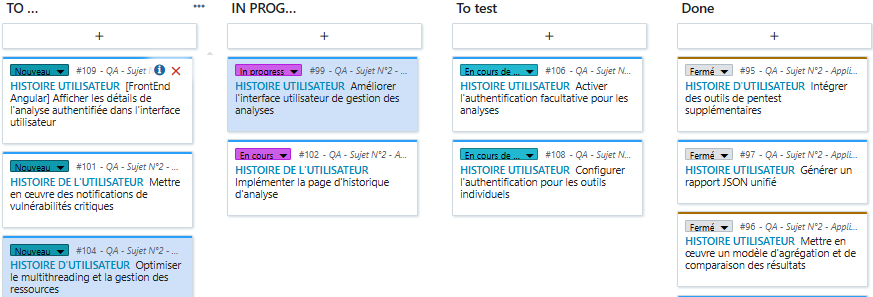
\includegraphics[width=\linewidth]{chapitres/ch2/img/board-sprit1.PNG}
    \caption{Scrum board Sprint 1}
    \label{fig:boardOpenProject}
\end{figure}
\vspace{-0.6cm}
\subsection{Burndown Chart}
Le Burndown Chart est un graphique visuel qui montre la quantité de travail terminée et celle restant à faire dans un sprint ou un projet, en fonction du temps écoulé. Il aide à estimer la capacité de l’équipe à atteindre ses objectifs dans les délais impartis et à détecter rapidement d’éventuelles dérives. La mise à jour régulière de ce graphique est essentielle pour anticiper les retards et ajuster le rythme de travail\cite{burndown}.

Nous avons généré les Burndown Charts à partir de l’avancement des tâches de chaque sprint. Ces graphiques nous ont permis de suivre efficacement notre progression et d’adapter notre charge de travail, comme illustré dans la figure \ref{fig:burndownChart} représentant le Burndown chart du projet.
\begin{figure}[H] 
    \centering 
    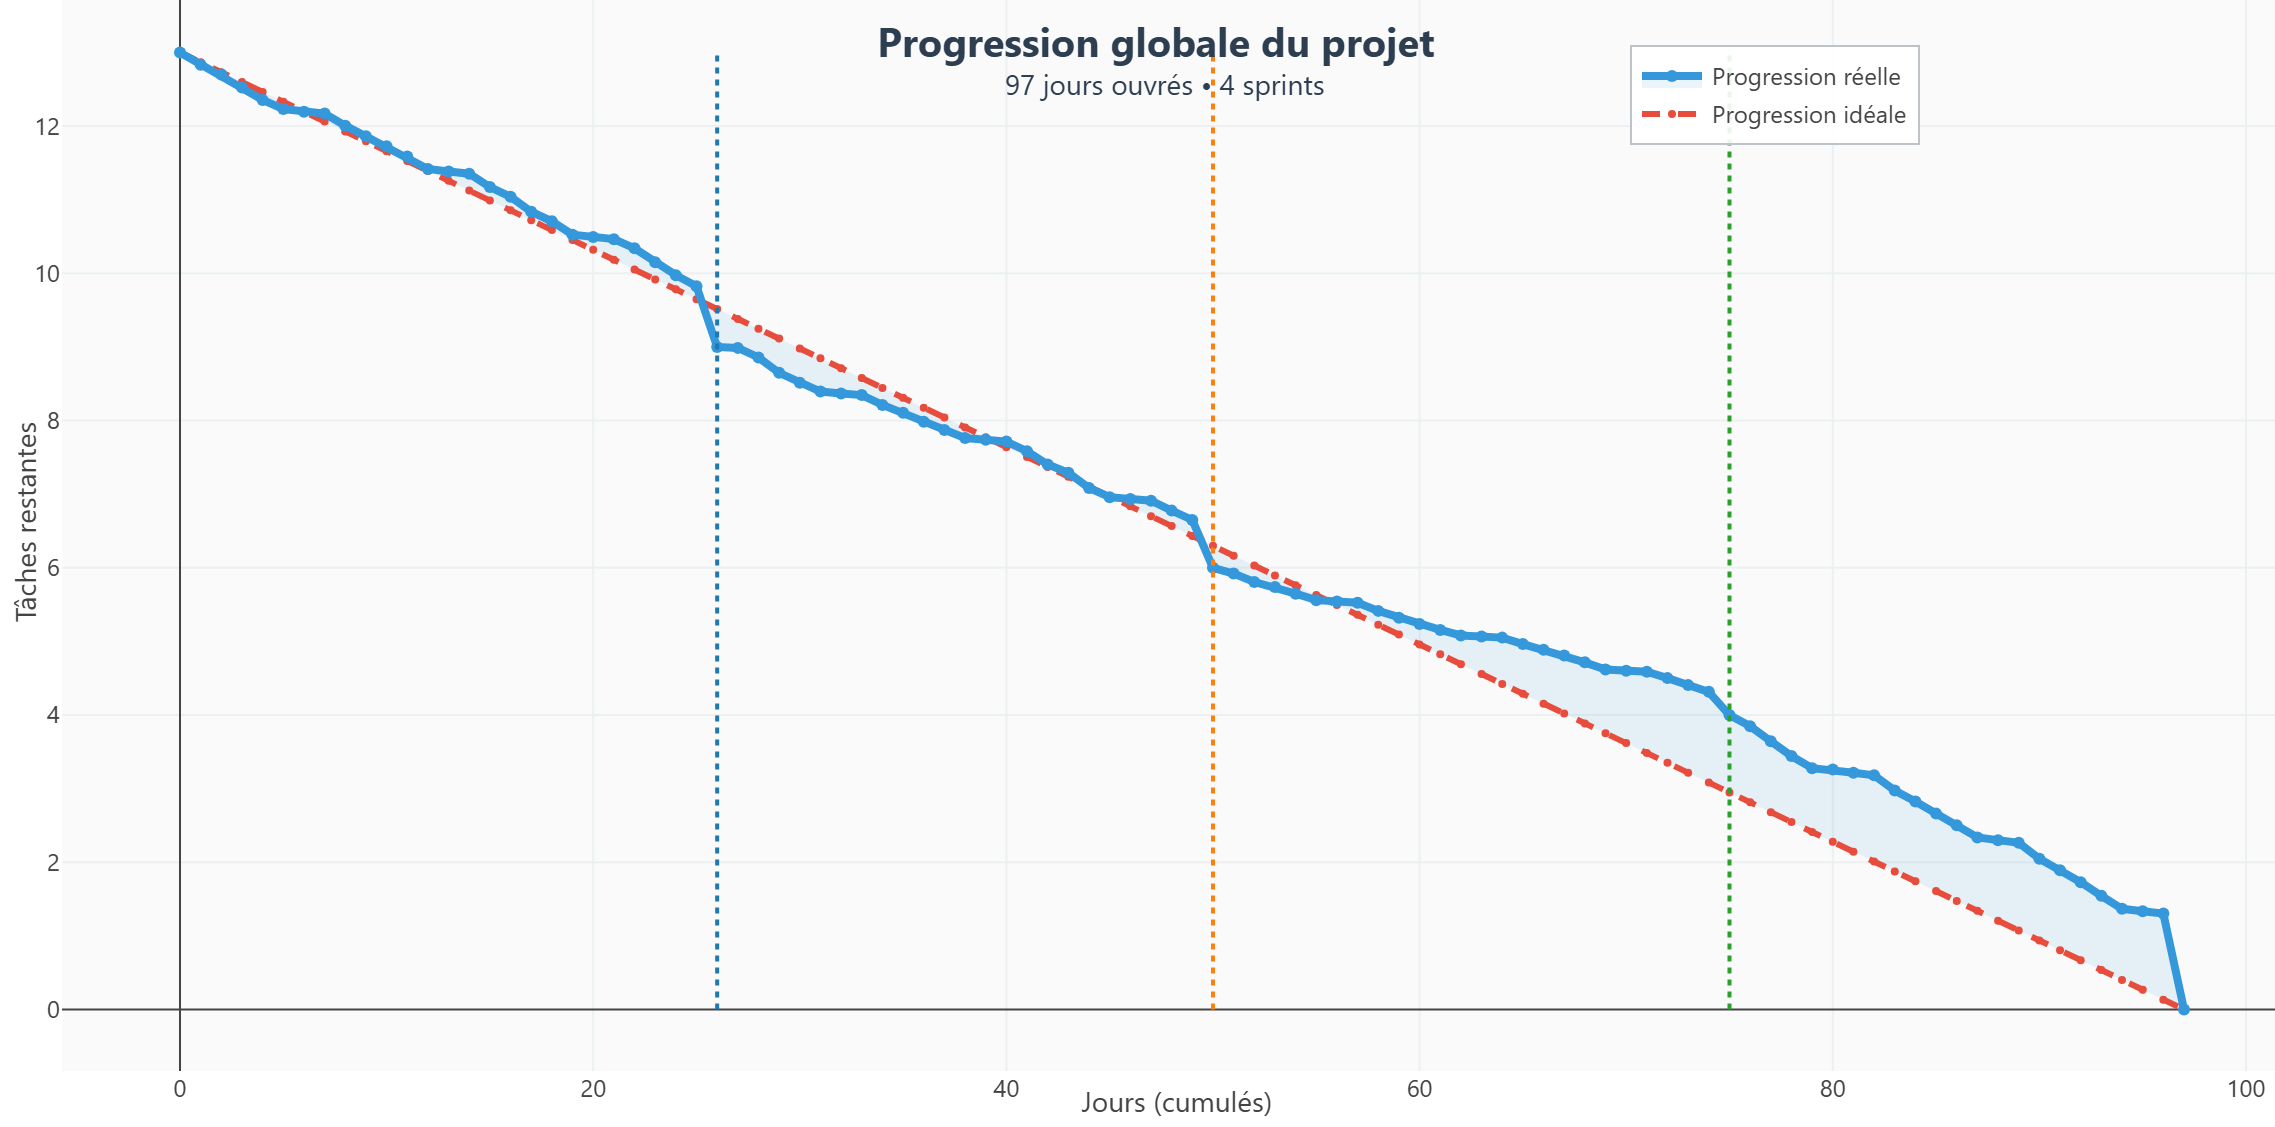
\includegraphics[width=0.97\linewidth]{chapitres/ch2/img/burndown.png} 
    \caption{Burndown chart projet} 
    \label{fig:burndownChart} \end{figure} 
\vspace{-0.8cm}
  
    \section{Environnement de développement}
    Cette section est dédiée pour la description de l’environnement matériel ainsi que l’environnement logiciel qui ont été employés pour la mise en œuvre de notre application
    \subsection{Environnement matériel}
    \begin{justify}
    Le tableau ~\ref{tab:environementMateriel} représente les caractéristiques techniques des machines utilisées pour la réalisation de notre application.
    \vspace{-0.5cm}
    \begin{table}[H]
        \begin{center}
        \renewcommand{\arraystretch}{1.5}
        \caption{Environnement matériel}
    	\begin{tabular}{|p{6cm}|p{8cm}|} 		
        	\hline				
        	\textbf{Type} & Ordinateur Portable\\\hline
            \textbf{Marque} & ASUS \\\hline
            \textbf{Processeur}  & Intel Core i5\\\hline
            \textbf{RAM} & 12 Go  \\ \hline
            \textbf{Disque dur} & 256 Go SSD\\\hline
            \textbf{Système d’exploitation}  & Windows 10 (64 bits)\\\hline
	      \end{tabular}
            \label{tab:environementMateriel}
        \end{center}
    \end{table}
\end{justify}
    \vspace{-0.5cm}
    \subsection{Environnement logiciel}
    \begin{justify}
    Pour la réalisation de notre application, plusieurs outils logiciels ont été utilisés, incluant les environnements de développement, les bibliothèques, les frameworks, ainsi que des outils et des services externes. Cette section présente une description de ces éléments.
    \subsubsection{Langages utilisés}
        Les langages présentés dans le tableau~\ref{tab:Langages} ont été utilisés pour développer les différentes composantes de l'application.
        \vspace{-0.3cm}
        \begin{spacing}{1.2}
            \begin{longtable}{|c|p{0.75\textwidth}|}
                \caption{Langages utilisés}
                \label{tab:Langages}\\
                \hline
                \textbf{Langage} & \textbf{Description} \\ \hline
                
                %% Python
                \begin{minipage}{0.2\textwidth}
                \centering
                    
\includegraphics[width=2cm]{chapitres/ch2/img/logiciel/python.png}
                \end{minipage}
                 & \begin{minipage}{0.75\textwidth} 
                  \justifying
                \vspace{0.2cm}
                \textbf{Python} est utilisé pour le développement du backend avec le framework \textbf{FastAPI}. Ce langage est reconnu pour sa lisibilité et sa simplicité, ce qui facilite la création d'API REST performantes et évolutives\cite{python}.
                \vspace{0.2cm}
                \end{minipage}\\ \hline
                
                %% TypeScript
                \begin{minipage}{0.2\textwidth}
                \centering
                    
\includegraphics[width=1.8cm]{chapitres/ch2/img/logiciel/ts.png}
                \end{minipage}
                 & \begin{minipage}{0.75\textwidth} 
                  \justifying
                \vspace{0.2cm}
                \textbf{TypeScript} est un sur-ensemble typé de JavaScript utilisé dans le développement de l'interface utilisateur via le framework \textbf{Angular}. Il permet de sécuriser le code et d'améliorer la maintenabilité des composants frontend\cite{typescript}.
                \vspace{0.2cm}
                \end{minipage}\\ \hline
    
                %% HTML
                \begin{minipage}{0.2\textwidth}
                \centering
                
\includegraphics[width=2cm]{chapitres/ch2/img/logiciel/html.png}
                \end{minipage}
                & \begin{minipage}{0.75\textwidth} 
                \justifying
                \vspace{0.2cm}
                \textbf{HTML (HyperText Markup Language)} est le langage standard utilisé pour structurer les pages web. Il définit les éléments de base tels que les titres, paragraphes, liens, tableaux, formulaires, etc.\cite{html}.
                \vspace{0.2cm}
                \end{minipage}\\ \hline
                
                %% CSS
                \begin{minipage}{0.2\textwidth}
                \centering
                
\includegraphics[width=2cm]{chapitres/ch2/img/logiciel/css.png}
                \end{minipage}
                & \begin{minipage}{0.75\textwidth} 
                \justifying
                \vspace{0.2cm}
                \textbf{CSS (Cascading Style Sheets)} est utilisé pour styliser les éléments HTML. Il permet de définir l'apparence des pages (couleurs, polices, marges, positionnement, etc.) afin d'améliorer l'expérience utilisateur\cite{css}.
                \vspace{0.2cm}
                \end{minipage}\\ \hline
                            %% SQL (PostgreSQL)
                \begin{minipage}{0.2\textwidth}
                    \centering
                        
\includegraphics[width=2cm]{chapitres/ch2/img/logiciel/sql.jpg}
                \end{minipage}
                 & \begin{minipage}{0.75\textwidth} 
                      \justifying
                        \vspace{0.2cm}
                        \textbf{SQL} est utilisé pour la gestion de la base de données relationnelle via le système \textbf{PostgreSQL}. Il permet de créer, manipuler et interroger les données de manière structurée\cite{postgresql}.
                        \vspace{0.2cm}
                \end{minipage}\\ \hline
                %% YAML
                \begin{minipage}{0.2\textwidth}
                    \centering
                        
\includegraphics[width=2cm]{chapitres/ch2/img/logiciel/yaml.png}
                \end{minipage}
                 & \begin{minipage}{0.75\textwidth} 
                    \justifying
                    \vspace{0.2cm}
                    \textbf{YAML} est utilisé pour la configuration des conteneurs dans \textbf{Docker Compose}. Il permet de définir les services, les volumes, les ports et les dépendances nécessaires au déploiement de l’application\cite{yaml}.
                    \vspace{0.2cm}
                \end{minipage}\\ \hline
                
                %% JSON
                \begin{minipage}{0.2\textwidth}
                    \centering
                        
\includegraphics[width=2cm]{chapitres/ch2/img/logiciel/json.jpg}
                \end{minipage}
                 & \begin{minipage}{0.75\textwidth} 
                    \justifying
                    \vspace{0.2cm}
                    \textbf{JSON (JavaScript Object Notation)} est utilisé comme format d'échange de données entre le frontend Angular et le backend FastAPI, ainsi que pour la documentation des API via Swagger/OpenAPI\cite{json}.
                    \vspace{0.2cm}
                \end{minipage}\\ \hline
                %% Bash
                \begin{minipage}{0.2\textwidth}
                    \centering
                        
\includegraphics[width=2cm]{chapitres/ch2/img/logiciel/bash.png}
                \end{minipage}
                 & \begin{minipage}{0.75\textwidth} 
                    \justifying
                    \vspace{0.2cm}
                    \textbf{Bash} est utilisé pour automatiser l'exécution de scripts liés aux tests de sécurité, au déploiement des conteneurs Docker, à la gestion des dépendances, et à l'enchaînement des outils d’analyse\cite{bash}.
                    \vspace{0.2cm}
                \end{minipage}\\ \hline
            \end{longtable}
        \end{spacing}
    \vspace{-0.2cm}
    \subsubsection{Logiciels utilisés}
    Le tableau~\ref{tab:Logiciels} présente un récapitulatif des outils employés pour la mise en œuvre de la solution ainsi que leurs descriptions.
    \vspace{-0.2cm}
            \begin{spacing}{1.1}
                \begin{longtable}{|c|p{0.75\textwidth}|}
                   \caption{Logiciels utilisés}
                    \label{tab:Logiciels}\\
                    \hline
                    \textbf{Logiciel} & \textbf{Description} \\ \hline
                    %% VS Code
                    \begin{minipage}{0.2\textwidth}
                    \centering
                        
\includegraphics[width=2.2cm]{chapitres/ch2/img/logiciel/vscode.png}
                    \end{minipage}
                     & \begin{minipage}{0.75\textwidth} 
                      \justifying
                    \vspace{0.2cm}
                    \textbf{Visual Studio Code (VS Code)} est un éditeur de code source open-source de Microsoft, réputé pour sa polyvalence, sa légèreté et ses fonctionnalités avancées. Il offre un environnement extensible grâce à des extensions, ce qui simplifie le travail des programmeurs\cite{VisualStudioCode}.\vspace{0.2cm}
                    \end{minipage}\\ \hline
                    %% GitHub
                    \begin{minipage}{0.2\textwidth}
                    \centering
                        
\includegraphics[width=3.2cm]{chapitres/ch2/img/logiciel/gitlab.png}
                    \end{minipage}
                     & \begin{minipage}{0.75\textwidth}
                      \justifying
                    \vspace{0.2cm}
                        \textbf{Gitlab} est une plateforme DevOps open source qui centralise le cycle de vie des projets logiciels : gestion de code, CI/CD, gestion de projet et sécurité. Elle favorise la collaboration, l’automatisation et la traçabilité, permettant aux équipes de planifier, développer, tester et déployer plus efficacement. Grâce à sa richesse fonctionnelle, elle s’impose comme un outil essentiel du développement moderne\cite{gitlab}.
                    \vspace{0.2cm}
                    \end{minipage}\\ \hline
                    %% Git
                    \begin{minipage}{0.2\textwidth}
                    \centering
                        
\includegraphics[width=2.1cm]{chapitres/ch2/img/logiciel/git.png}
                    \end{minipage}
                     & \begin{minipage}{0.75\textwidth} 
                     \justifying
                    \vspace{0.2cm}
                        \textbf{Git} permet la gestion efficace des branches pour travailler simultanément sur plusieurs projets sans conflits, en offrant une interface console conviviale, des algorithmes de fusion intelligents pour gérer les modifications simultanées de fichiers\cite{git}.
                    \vspace{0.2cm}
                    \end{minipage}\\ \hline
                    %% Docker Desktop
                    \begin{minipage}{0.2\textwidth}
                    \centering
                        
\includegraphics[width=2.6cm]{chapitres/ch2/img/logiciel/Docker Desktop.png}
                    \end{minipage}
                     & \begin{minipage}{0.75\textwidth} 
                      \justifying
                    \vspace{0.2cm}
                    \textbf{Docker Desktop} est une application pour Windows, macOS et Linux qui fournit une interface utilisateur graphique (GUI) pour gérer les conteneurs, images et réseaux Docker localement. Elle inclut Docker Engine, Docker CLI, Docker Compose, Kubernetes et d'autres outils utiles pour le développement et le test de conteneurs\cite{dockerdesktop}.
                    \vspace{0.2cm}
                    \end{minipage}\\ \hline
                    %% WebSocket
                    \begin{minipage}{0.2\textwidth}
                    \centering
                        
\includegraphics[width=2cm]{chapitres/ch2/img/logiciel/websocket.png}
                    \end{minipage}
                     & \begin{minipage}{0.75\textwidth} 
                      \justifying
                    \vspace{0.2cm}
                    \textbf{WebSocket} est un protocole de communication bidirectionnelle full-duplex permettant des échanges en temps réel entre client et serveur. Il est utilisé pour transmettre en direct les résultats des scans et notifier l’utilisateur via l’interface Angular\cite{websocket}.
                    \vspace{0.2cm}
                    \end{minipage}\\ \hline
                    %% Overleaf
                    \begin{minipage}{0.2\textwidth}
                    \vspace{0.2cm}
                    \centering
                        
\includegraphics[width=2.2cm]{chapitres/ch2/img/logiciel/overleaf.png}
                    \end{minipage}
                     & \begin{minipage}{0.75\textwidth}
                      \justifying
                    \vspace{0.2cm}
                         \textbf{Overleaf} est une plateforme en ligne de rédaction collaborative en temps réel de documents LaTeX, conçue pour la création de documents scientifiques, académiques et techniques\cite{Overleaf}.
                    \vspace{0.2cm}
                    \end{minipage}\\ \hline
                    %% StarUML
                    \begin{minipage}{0.2\textwidth}
                    \centering
                        
\includegraphics[width=1.9cm]{chapitres/ch2/img/logiciel/staruml.png}
                    \end{minipage}
                     & \begin{minipage}{0.75\textwidth} 
                      \justifying
                    \vspace{0.2cm}
                         \textbf{StarUML} est un logiciel de modélisation UML utilisé pour concevoir des diagrammes pour la conception de logiciels. Il offre des fonctionnalités de modélisation avancées pour les concepteurs de logiciels\cite{StarUML}. \vspace{0.2cm}
                    \end{minipage}\\ \hline
                    %% Trello
                    \begin{minipage}{0.2\textwidth}
                    \centering
                        
\includegraphics[width=3cm]{chapitres/ch2/img/logiciel/openproject.png}
                    \end{minipage}
                     & \begin{minipage}{0.75\textwidth}
                      \justifying
                        \vspace{0.2cm}
                         \textbf{OpenProject} est un logiciel de gestion de projet open source conçu pour être utilisé avec des méthodologies de gestion de projet traditionnelles, mais aussi dans un environnement agile ou une méthodologie hybride. Collaboratif, il offre un suivi de projet et une suite complète de fonctionnalités permettant de gérer des projets complexes\cite{openproject}.
                    \vspace{0.2cm}
                    \end{minipage}\\ \hline
                    %% Postman
                    \begin{minipage}{0.2\textwidth}
                    \centering
                        
\includegraphics[width=2.2cm]{chapitres/ch2/img/logiciel/postman.png}
                    \end{minipage}
                     & \begin{minipage}{0.75\textwidth} 
                      \justifying
                    \vspace{0.2cm}
                         \textbf{Postman} est un outil de développement d'API qui permet aux développeurs de tester, de documenter et de surveiller les API de manière efficace. Il offre une interface conviviale pour créer des requêtes HTTP, automatiser des tests et collaborer sur des projets d'API \cite{Postman}.
                    \vspace{0.2cm}
                    \end{minipage}\\ \hline
            
            
                    \begin{minipage}{0.2\textwidth}
                    \centering
                        
\includegraphics[width=2.2cm]{chapitres/ch2/img/logiciel/Swagger.png}
                    \end{minipage}
                     & \begin{minipage}{0.75\textwidth} 
                      \justifying
                    \vspace{0.2cm}
                        \textbf{Swagger} est un langage de description d’interface permettant de définir des API REST à l’aide du format JSON. Il s’appuie sur la spécification OpenAPI, qui standardise la description de la structure d’une API. Il permet de concevoir, documenter, tester et consommer des API REST facilitant ainsi la compréhension et l’intégration des services web\cite{Swagger}.
                    \vspace{0.2cm}
                    \end{minipage}\\ \hline
            
                \begin{minipage}{0.2\textwidth}
                    \centering
                        
\includegraphics[width=2.2cm]{chapitres/ch2/img/logiciel/Selenium.png}
                    \end{minipage}
                     & \begin{minipage}{0.75\textwidth} 
                      \justifying
                    \vspace{0.2cm}
                        \textbf{Selenium} est un outil open-source largement utilisé pour l'automatisation des tests des applications web. Il permet d'écrire des scripts de test dans divers langages de programmation comme Java, Python, C\#. Il permet de simuler des interactions utilisateur telles que les clics, la saisie de texte et la navigation entre les pages, ce qui est essentiel pour les tests fonctionnels des applications web.\cite{selenium}.
                    \vspace{0.2cm}
                    \end{minipage}\\ \hline
                \end{longtable}
            \end{spacing}
            \vspace{-0.1cm}
    \subsubsection{ Frameworks utilisées}
    Le tableau~\ref{tab:Libs} présente les principales  frameworks utilisées dans le développement de l'application, réparties entre le backend et le frontend. Ces  frameworks  ont permis de faciliter le développement, d'améliorer les performances et de garantir la sécurité et la maintenabilité du projet.
    \begin{spacing}{1.1}
        \begin{longtable}{|c|p{0.75\textwidth}|}
            \caption{Bibliothèques utilisées}
            \label{tab:Libs}\\
            \hline
            \textbf{Bibliothèque} & \textbf{Description} \\ \hline
            
            %% FastAPI
            \begin{minipage}{0.2\textwidth}
                \centering
                    
\includegraphics[width=1.9cm]{chapitres/ch2/img/logiciel/fastapi.png}
            \end{minipage}
             & \begin{minipage}{0.75\textwidth} 
                \justifying
                \vspace{0.2cm}
                \textbf{FastAPI} est une bibliothèque Python moderne permettant de créer des API web de manière rapide, performante et avec une documentation automatique générée via OpenAPI/Swagger\cite{fastapi}.
                \vspace{0.2cm}
            \end{minipage}\\ \hline
            
            %% Angular 
            \begin{minipage}{0.2\textwidth}
                \centering
                    
\includegraphics[width=2.6cm]{chapitres/ch2/img/logiciel/angular.png}
            \end{minipage}
             & \begin{minipage}{0.75\textwidth} 
                    \justifying
                    \vspace{0.2cm}
                    \textbf{Angular} est un framework de développement frontend basé sur TypeScript, utilisé pour concevoir des applications web dynamiques, modulaires et performantes. Il propose une architecture robuste fondée sur des composants, un système de routage, des formulaires réactifs ainsi qu’une gestion d’état, facilitant le développement d’interfaces utilisateur complexes \cite{angular}.
                    \vspace{0.1cm}
            \end{minipage}\\ \hline
            
            %% Bootstrap
            \begin{minipage}{0.2\textwidth}
                \centering
                
\includegraphics[width=2cm]{chapitres/ch2/img/logiciel/bootstrap.jpg}
                \end{minipage}
                & \begin{minipage}{0.75\textwidth} 
                \justifying
                \vspace{0.2cm}
                \textbf{Bootstrap} est une bibliothèque CSS open-source qui facilite le développement de sites web réactifs. Elle fournit des composants préconçus (boutons, cartes, grilles) et garantit une compatibilité multi-appareils\cite{bootstrap}.
                \vspace{0.2cm}
                \end{minipage}\\ \hline
            \end{longtable}
        \end{spacing}
    \vspace{-0.1cm}
    \subsubsection{Outils de sécurité utilisés}
    Le tableau~\ref{tab:OutilsSecurite} présente les outils de sécurité employés pour les tests de vulnérabilités et l'analyse de sécurité de l'application.
    \begin{spacing}{1.1}
        \begin{longtable}{|c|p{0.75\textwidth}|}
            \caption{Outils de sécurité utilisés}
            \label{tab:OutilsSecurite}\\
            \hline
            \textbf{Outil} & \textbf{Description} \\ \hline
            
            %% ZAP
            \begin{minipage}{0.2\textwidth}
                \centering
                    
\includegraphics[width=2.4cm]{chapitres/ch2/img/tools/zap.png}
            \end{minipage}
             & \begin{minipage}{0.75\textwidth} 
                \justifying
                \vspace{0.2cm}
                \textbf{ZAP (OWASP Zed Attack Proxy)} est un outil open-source de test de sécurité des applications web. Il permet de détecter automatiquement les vulnérabilités courantes telles que les failles XSS (Cross-Site Scripting), CSRF (Cross-Site Request Forgery), et les injections SQL dans les applications web\cite{zap}.
                \vspace{0.2cm}
            \end{minipage}\\ \hline
            
            %% SQLMap
            \begin{minipage}{0.2\textwidth}
                \centering
                    
\includegraphics[width=3.4cm]{chapitres/ch2/img/tools/sqlmap.png}
            \end{minipage}
             & \begin{minipage}{0.75\textwidth} 
                \justifying
                \vspace{0.2cm}
                \textbf{SQLMap} est un outil automatisé open-source spécialisé dans la détection et l'exploitation des vulnérabilités d'injection SQL. Il prend en charge de nombreux systèmes de gestion de bases de données et offre des techniques avancées pour l'extraction de données et la prise de contrôle des bases de données vulnérables\cite{sqlmap}.
                \vspace{0.2cm}
            \end{minipage}\\ \hline
            
            %% Wapiti
            \begin{minipage}{0.2\textwidth}
                \centering
                    
\includegraphics[width=2.8cm]{chapitres/ch2/img/tools/wapiti.png}
            \end{minipage}
             & \begin{minipage}{0.75\textwidth} 
                \justifying
                \vspace{0.2cm}
                \textbf{Wapiti} est un scanner de vulnérabilités web open-source qui effectue des audits de sécurité en analysant les pages web pour détecter les scripts et les formulaires où il pourrait injecter des données. Il permet d'identifier diverses vulnérabilités comme les injections SQL, XSS, et les inclusions de fichiers\cite{wapiti}.
                \vspace{0.2cm}
            \end{minipage}\\ \hline
            
            %% Nikto
            \begin{minipage}{0.2\textwidth}
                \centering
                    
\includegraphics[width=2.4cm]{chapitres/ch2/img/tools/nikto.png}
            \end{minipage}
             & \begin{minipage}{0.75\textwidth} 
                \justifying
                \vspace{0.2cm}
                \textbf{Nikto} est un scanner de vulnérabilités web open-source qui effectue des tests complets contre les serveurs web pour multiple vulnérabilités, incluant plus de 6700 fichiers/programmes potentiellement dangereux, les versions obsolètes de serveurs, et les problèmes de configuration spécifiques aux serveurs\cite{nikto}.
                \vspace{0.2cm}
            \end{minipage}\\ \hline
            
            %% Nuclei
            \begin{minipage}{0.2\textwidth}
                \centering
                    
\includegraphics[width=3.2cm]{chapitres/ch2/img/tools/nuclei.png}
            \end{minipage}
             & \begin{minipage}{0.75\textwidth} 
                \justifying
                \vspace{0.2cm}
                \textbf{Nuclei} est un scanner de vulnérabilités rapide et personnalisable basé sur des templates YAML. Il permet d'effectuer des scans de sécurité à grande échelle avec une approche modulaire, supportant la détection de diverses vulnérabilités web, réseau et cloud\cite{nuclei}.
                \vspace{0.2cm}
            \end{minipage}\\ \hline
            
            %% Nmap
            \begin{minipage}{0.2\textwidth}
                \centering
                    
\includegraphics[width=2.8cm]{chapitres/ch2/img/tools/nmap.png}
            \end{minipage}
             & \begin{minipage}{0.75\textwidth} 
                \justifying
                \vspace{0.2cm}
                \textbf{Nmap (Network Mapper)} est un outil open-source de découverte réseau et d'audit de sécurité. Il permet de scanner les ports ouverts, identifier les services en cours d'exécution, détecter les systèmes d'exploitation, et effectuer des scripts de reconnaissance avancés sur les réseaux\cite{nmap}.
                \vspace{0.2cm}
            \end{minipage}\\ \hline
            
            %% XSStrike
            \begin{minipage}{0.2\textwidth}
                \centering
                    
\includegraphics[width=2.4cm]{chapitres/ch2/img/tools/XSStrike.png}
            \end{minipage}
             & \begin{minipage}{0.75\textwidth} 
                \justifying
                \vspace{0.2cm}
                \textbf{XSStrike} est un outil avancé de détection des vulnérabilités Cross-Site Scripting (XSS). Il utilise des techniques de fuzzing intelligentes et une analyse contextuelle pour identifier les failles XSS complexes que les scanners traditionnels pourraient manquer\cite{xsstrike}.
                \vspace{0.2cm}
            \end{minipage}\\ \hline
            
            %% PwnXSS
            \begin{minipage}{0.2\textwidth}
                \centering
                    
\includegraphics[width=3.6cm]{chapitres/ch2/img/tools/PwnXSS.png}
            \end{minipage}
             & \begin{minipage}{0.75\textwidth} 
                \justifying
                \vspace{0.2cm}
                \textbf{PwnXSS} est un outil spécialisé dans la détection avancée des vulnérabilités Cross-Site Scripting. Il offre des capacités de scanning automatisé avec des payloads personnalisés et une analyse approfondie des réponses pour identifier les failles XSS dans diverses configurations d'applications web\cite{pwnxss}.
                \vspace{0.2cm}
            \end{minipage}\\ \hline
            
            %% WafW00f
            \begin{minipage}{0.2\textwidth}
                \centering
                    
\includegraphics[width=2.4cm]{chapitres/ch2/img/tools/wafw00f.png}
            \end{minipage}
             & \begin{minipage}{0.75\textwidth} 
                \justifying
                \vspace{0.2cm}
                \textbf{WafW00f} est un outil Python conçu pour identifier et fingerprinter les Web Application Firewalls (WAF) protégeant une application web. Il permet aux testeurs de sécurité de déterminer la présence et le type de WAF afin d'adapter leurs stratégies de test en conséquence\cite{wafw00f}.
                \vspace{0.2cm}
            \end{minipage}\\ \hline
            
            %% WhatWeb
            \begin{minipage}{0.2\textwidth}
                \centering
                    
\includegraphics[width=3.6cm]{chapitres/ch2/img/tools/Whatweb.png}
            \end{minipage}
             & \begin{minipage}{0.75\textwidth} 
                \justifying
                \vspace{0.2cm}
                \textbf{WhatWeb} est un outil de reconnaissance web qui identifie les technologies utilisées par un site web, incluant les systèmes de gestion de contenu, les frameworks, les serveurs web, les bibliothèques JavaScript, et d'autres composants technologiques. Il est essentiel pour le fingerprinting et la reconnaissance passive\cite{whatweb}.
                \vspace{0.2cm}
            \end{minipage}\\ \hline
        \end{longtable}
    \end{spacing}
    \vspace{-0.1cm}
    \subsubsection{Système de gestion de base de données : PostgreSQL}
        \begin{minipage}{0.25\textwidth}
            \centering
            
\includegraphics[width=3cm]{chapitres/ch2/img/logiciel/postgresql.png}
        \end{minipage}
        \begin{minipage}{0.75\textwidth} 
            \justifying
            \textbf{PostgreSQL} est un système de gestion de base de données relationnelle (SGBDR) open-source reconnu pour sa robustesse, sa conformité aux standards SQL, et son extensibilité. Il est utilisé pour stocker les données de manière fiable, en assurant l'intégrité des transactions, la cohérence et la sécurité des informations.
        \end{minipage}
        
        Dans notre application, PostgreSQL permet de gérer les entités principales telles que les utilisateurs, les messages, les enregistrements de données, etc. Il est accédé via SQLAlchemy, un ORM Python, facilitant les interactions entre les objets du backend (FastAPI) et la base de données.
    \subsubsection{Système de gestion des files de messages : RabbitMQ}
        \begin{minipage}{0.25\textwidth}
            \centering
            
\includegraphics[width=3cm]{chapitres/ch2/img/logiciel/rabbitmq.png}
        \end{minipage}
        \begin{minipage}{0.75\textwidth} 
            \justifying
            \textbf{RabbitMQ} est un broker de messages open-source basé sur le protocole AMQP, permettant une communication asynchrone entre microservices et composants distribués. Il facilite le traitement parallèle ainsi que la gestion des files d’attente dans l’architecture backend \cite{rabbitmq}.
        \end{minipage}
        
        Dans notre application, RabbitMQ gère la mise en file d’attente des tâches de scans de sécurité afin d’améliorer les performances en limitant le nombre de scans exécutés simultanément et en évitant la surcharge des ressources. Les requêtes de scan sont placées dans des queues puis consommées par des workers dédiés, ce qui garantit une exécution efficace, fiable et scalable. Cette architecture favorise la tolérance aux pannes, le traitement asynchrone et l’extensibilité future. L’intégration s’appuie sur la bibliothèque Python \texttt{pika}, connectée au backend FastAPI, qui orchestre la production et la consommation des messages. Ainsi, les producteurs (backend FastAPI) envoient les requêtes de scan vers RabbitMQ, tandis que les consommateurs (workers) traitent ces messages en parallèle, optimisant la gestion de la charge et les performances.
\end{justify} 
    \section{Architecture de l’application}
    Cette section présente l’architecture de notre solution, conçue pour garantir la cohérence, la performance, la maintenabilité et la scalabilité de l’application. Elle repose sur une architecture en trois tiers, typique des applications web modernes, intégrant des services conteneurisés et orchestrés afin d’optimiser le développement, le déploiement et l’exécution.

L’architecture s’articule autour de trois couches principales:
\begin{itemize}[label=$-$]
    \item \textbf{Couche de présentation (Frontend)}: développée avec \textbf{Angular} (version 18), cette couche constitue l’interface utilisateur accessible via un navigateur web, sur le port \textbf{4200}. L’application est conteneurisée à l’aide de \textbf{Docker} et servie par un serveur web \textbf{NGINX} sur le port \textbf{80}, garantissant rapidité et sécurité côté client. Elle suit le modèle \textbf{\acs{MVVM}} (Model-View-ViewModel)\cite{mvvm}:
            \begin{itemize}[label=$\circ$]
                    \item \textbf{Model}: définit les structures de données via des interfaces \texttt{TypeScript}, représentant les entités métier (utilisateurs, scans, résultats...).
                    \item \textbf{View}: composants visuels construits en \texttt{HTML}/\texttt{CSS}, correspondant à la partie graphique de l’application.
                    \item \textbf{ViewModel}: représenté par les \textbf{Components} Angular (liaison entre données et vue) et les \textbf{Services} (logique métier côté client, communication avec le backend).
            \end{itemize}
        En complément, le frontend s’appuie sur plusieurs mécanismes clés assurant la sécurité, la modularité et l’interactivité de l’application:
        \begin{itemize}[label=$\circ$]
            \item \textbf{Guards et routing Angular}: sécurisent la navigation à travers un système de routes hiérarchisées, protégées selon l’état d’authentification et le rôle de l’utilisateur.
            \item \textbf{Services Angular}: centralisent les interactions avec l’API REST (via \texttt{HttpClient}) et les traitements locaux (authentification, stockage, notifications, WebSocket).
            \item \textbf{Modèles TypeScript}: définissent les formats d’échange avec le backend, alignés avec les schémas \texttt{Pydantic} de FastAPI, pour faciliter la sérialisation/désérialisation des données.
            \item \textbf{WebSocket}: permet une communication bidirectionnelle en temps réel pour recevoir les mises à jour instantanées (progression des scans, alertes système).
        \end{itemize}
    \item \textbf{Couche applicative (Backend)}: développée avec \textbf{FastAPI}, elle est accessible via le port \textbf{8000} pour les requêtes \acs{HTTP}, et le port \textbf{8001} pour les communications \textbf{WebSocket}. Elle assure la logique métier, le traitement des requêtes, l’exposition des services web REST, l’interfaçage avec la base de données, la gestion de l’authentification et la coordination entre les autres couches.
    L’application est conteneurisée à l’aide de \textbf{Docker} et déployée via un \textbf{serveur Uvicorn} conforme à l’interface \textbf{\acs{ASGI}}, utilisé pour exécuter l’application \textbf{FastAPI}. Ce serveur gère efficacement les requêtes \acs{HTTP}/\acs{HTTPS} et les transmet aux routes définies dans FastAPI. Il prend également en charge les communications asynchrones via les \textbf{WebSockets}, ce qui le rend particulièrement adapté aux applications modernes nécessitant des échanges en temps réel.
    \begin{enumerate}[left=-0.03cm]
        \item \textbf{Les composants principaux de fastapi sont\cite{fastapiArc}}:
            \begin{itemize}[label=$\bullet$, left=-0.08cm]
                \item \textbf{Routes:} définissent les points d'entrée de l'\acs{API} REST, organisés par fonctionnalité et reçoivent les requêtes \acs{HTTP}.
                \item \textbf{CRUD}: Contiennent la logique métier et le traitement des données.
                \item \textbf{Models:} représentent les entités de la base de données sous forme de classes SQLAlchemy (\acs{ORM}).
                \item \textbf{Schemas Pydantic:} utilisés pour la validation et la sérialisation des données, ils définissent la structure des informations échangées (requêtes et réponses) entre le client et l’API.
                \item \textbf{\acs{DAO} (Data Access Objects)}: basé sur \textbf{SQLAlchemy} pour accéder à la base de données PostgreSQL, en assurant le mapping objet-relationnel (ORM).
                \item \textbf{JWT / OAuth2:} mécanisme d’authentification sécurisé reposant sur l’utilisation de \textbf{\acs{JWT}} (JSON Web Tokens) en combinaison avec le protocole \textbf{\acs{OAuth2}}, permettant la gestion des sessions, le contrôle des accès et l’attribution des rôles utilisateurs.
                \item \textbf{Canal WebSocket}: utilisé pour la communication en temps réel avec les utilisateurs, il permet à ces derniers de recevoir des mises à jour instantanées (notifications, état des scans, messages système...).
            \end{itemize}
        \item \textbf{Composants spécifiques ajoutés pour ce projet:}
            \begin{itemize}[label=$\bullet$, left=-0.08cm]
                \item \textbf{File de messages RabbitMQ + Workers}: fonctionne sur le port \textbf{5672} (port par défaut pour le protocole \acs{AMQP}) et expose une interface d’administration sur le port \textbf{15672}. Ce système permet le traitement asynchrone des tâches lourdes, telles que la gestion des scans, en répartissant la charge entre un pool de \textbf{workers asynchrones}. Les requêtes sont placées dans une file d’attente, puis traitées selon un nombre limité de tâches concurrentes afin de garantir les performances et la stabilité du système.\\
                Ce mécanisme permet de:
                \begin{itemize}[label=$\circ$]
                    \item Enregistrer les requêtes de scan dans RabbitMQ.
                    \item Traiter les tâches de façon asynchrone via un nombre fixe de \textbf{workers}.
                    \item Garantir une répartition équitable des ressources (N scans simultanés maximum).
                    \item Notifier l’utilisateur en temps réel une fois le traitement terminé.
                \end{itemize}
                Il favorise ainsi la scalabilité et prévient la saturation du système.
                \item \textbf{Service \acs{SMTP}}: utilisé pour l’envoi d’e-mails via le port \textbf{587} (TLS), selon la configuration du serveur SMTP.
                \item \textbf{Intégration \acs{Slack}}: notifications automatiques envoyées sur un canal Slack configuré via Webhook pour informer en temps réel des événements critiques (début/fin de scan, erreurs, vulnérabilités détectées).
                \item \textbf{Intégration Jira}: création automatique de tickets dans Jira lors de la détection de vulnérabilités critiques ou bloquantes, avec transmission des détails techniques (type, niveau de risque, description, solution proposée) depuis le backend.
               \item \textbf{Outils de sécurité}: L’application intègre plusieurs outils de scan automatisé, chacun exécuté dans un conteneur \textbf{Docker} isolé afin de garantir la modularité et l’évolutivité. Parmi ces outils, OWASP ZAP est accessible via le port \textbf{8080}, utilisé pour l’API et le proxy web. Les autres outils SQLMap, Wapiti, Nikto, Nuclei, Nmap, XSStrike, PwnXSS, WafW00f et WhatWeb sont lancés via des commandes dans leurs conteneurs Docker respectifs, sans ports exposés, car ils ne fonctionnent pas comme des services persistants. Les résultats sont ensuite centralisés, structurés et unifiés afin de pouvoir être exploités par d’autres modules tels que l’affichage, le reporting ou les alertes.
                \item \textbf{Outils pour les tests fonctionnels et audits SEO automatisés}:  
                    \begin{itemize}[label=$\circ$]
                        \item \textbf{Selenium}: utilisé pour simuler des interactions complexes avec des navigateurs web (navigation authentifiée, clics, remplissage de formulaires) afin de vérifier le comportement fonctionnel de l’application. Exécuté via un conteneur (\texttt{selenium/standalone-chrome}) sur le port \textbf{4444} (WebDriver).
                        \item \textbf{BeautifulSoup}: bibliothèque Python, utilisé pour analyser le DOM des pages web, permettant de détecter les balises et attributs essentiels à l’indexation (titres, meta description, balises \textit{alt}, structure \acs{HTML}...).
                    \end{itemize}                
            \end{itemize}
    \end{enumerate}
    \item \textbf{Couche de données}: assurée par une base de données relationnelle \textbf{PostgreSQL}, accessible via le port \textbf{5432}, elle stocke l’ensemble des informations de l’application, telles que les comptes utilisateurs, les résultats des scans, les historiques et les notifications. L’accès aux données est réalisé via des modèles \textbf{ORM (SQLAlchemy)}, garantissant la cohérence entre les entités logicielles et les tables relationnelles.
\end{itemize}
\noindent Tous les services (Angular, FastAPI, PostgreSQL, RabbitMQ, WebSocket...) sont conteneurisés avec \textbf{Docker} et orchestrés via \textbf{Docker Compose}, utilisant un réseau virtuel interne (bridge Docker) pour assurer une communication fluide entre les conteneurs.

La figure \ref{fig:architecture} illustre l’architecture de notre application en mettant en évidence les interactions entre ses différentes couches.
\begin{figure}[H]
    \centering
    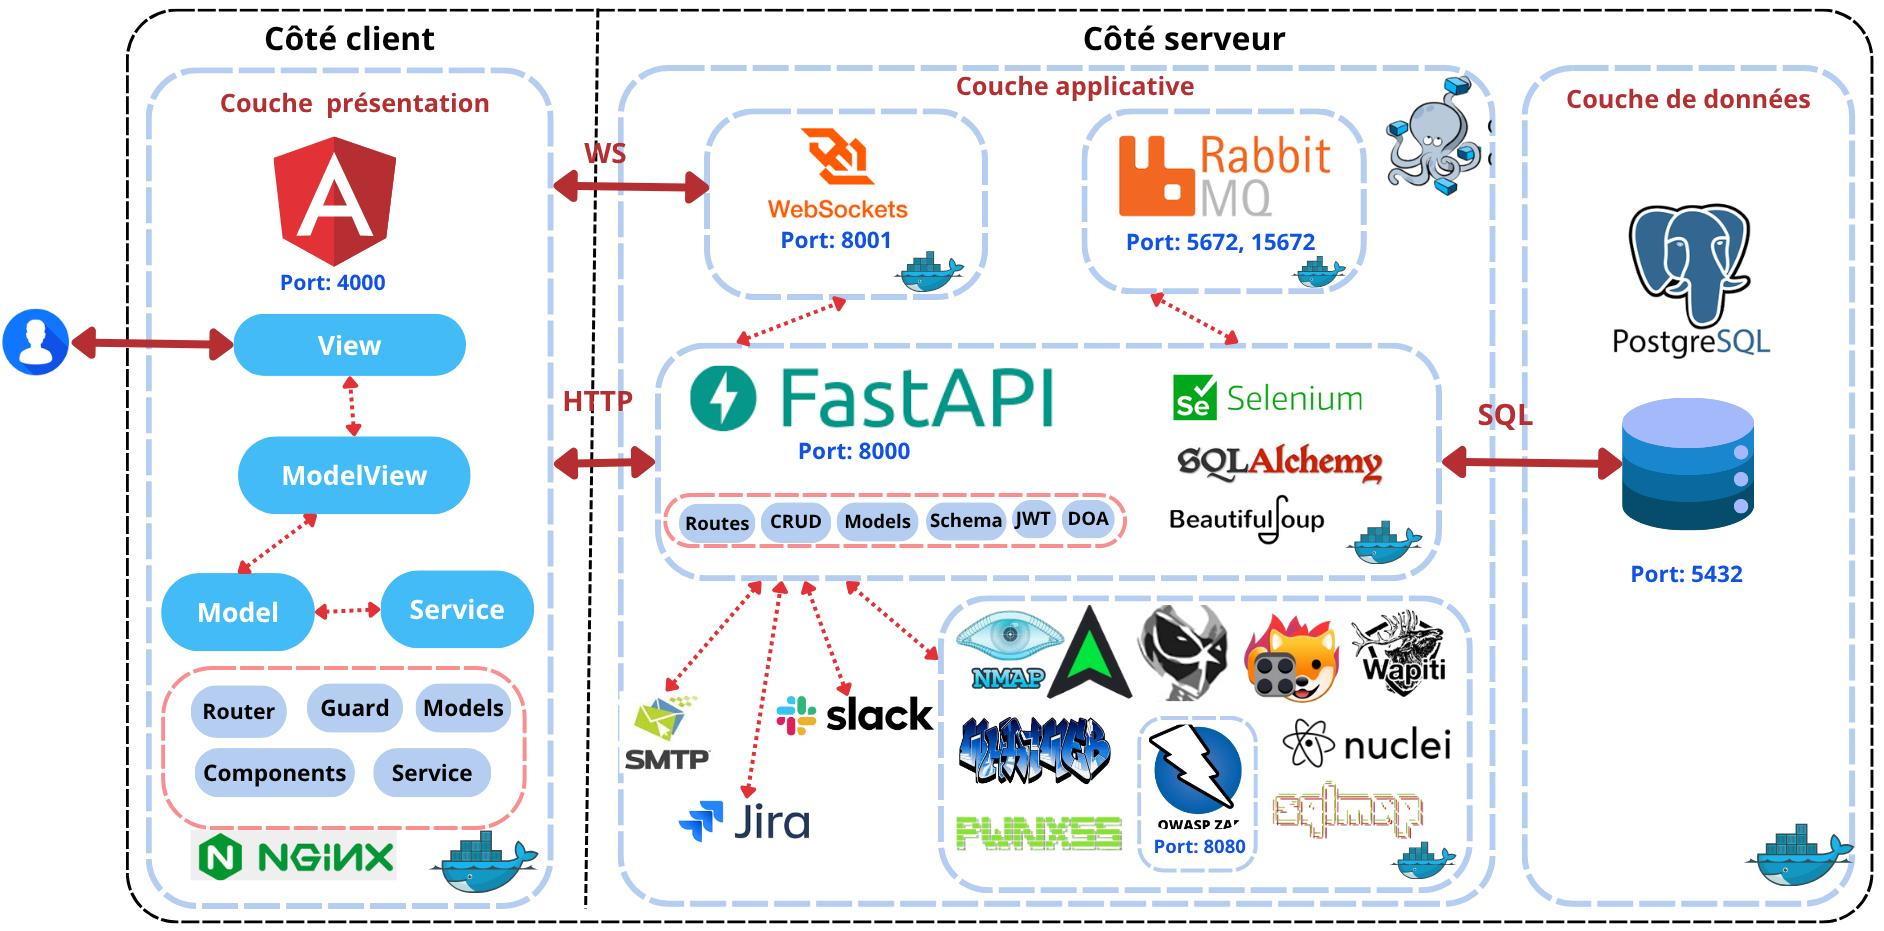
\includegraphics[width=\linewidth]{chapitres/ch2/img/architecture.png}
    \caption{Architecture de l’application}
    \label{fig:architecture}
\end{figure}
\vspace{-0.8cm}
\noindent Cette architecture conteneurisée garantit une haute disponibilité, la sécurité et la performance du système. Elle facilite la maintenance et l’évolution du projet, tout en assurant une scalabilité grâce à une séparation claire des responsabilités et à l’utilisation de services indépendants.
    \section*{\texorpdfstring{Conclusion}{Conclusion}}
    \addcontentsline{toc}{chapter}{\textbf{Conclusion}}
    \input{chapitres/ch2/section/Conclusion}
\end{justify}